\section{Theory of Operations}

\subsection{Introduction}
The \textbf{Dff} is a basic D flip-flop with a parameterized width.

\begin{figure}[h]
  \centering
  \includegraphics[scale=.75]{images/dff.io.drawio.png}
  \caption{Block Diagram}\label{fig:block-diagram}
\end{figure}

\newpage
\subsection{Interface Timing}

Data on the input \textbf{d} will appear on the output \textbf{q} on the following clock cycle if \textbf{enable} is asserted. If \textbf{enable} is not asserted, \textbf{q} will retain its current state on the next clock cycle. The timing diagram shown below in Figure~\ref{fig:timing} represents an instantiation with the following parameters.

\begin{lstlisting}[language=Scala]
val myRegister = new Dff(width = 8) 
\end{lstlisting}

\begin{figure}[h]
  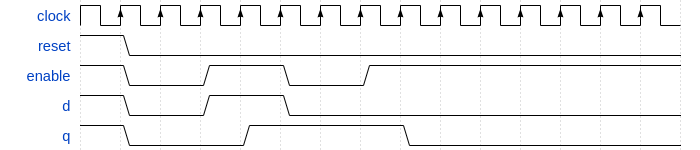
\includegraphics[width=\textwidth]{images/Dff.wavedrom.png}
  \caption{Timing Diagram}\label{fig:timing}
\end{figure}